%\vspace{1.5pc}
\vspace{1.5pc}
%\section[State of the Art]{State of the Art}
\vspace{-1pc}
\section[Penelitian Terkait IOD]{Penelitian Terkait IOD}
\begin{spacing}{1.5}
	Hasil analisis data observasi selama 40 tahun (1958-1997) menunjukkan fenomena mode dipol di Samudera Hindia. Pola variasi internal dengan anomali \textit{sea surface temperature} (SST) rendah di sekitar Sumatra dan tinggi di sebelah barat Samudera Hindia, disertai dengan angin dan presipitasi. Keterkaitan spasial-temporal antara SST dan angin kuat melalui medan presipitasi dan dinamika laut. Proses interaksi udara-laut ini unik dan terbukti independen dari fenomena osilasi selatan El Nino (ENSO). Penemuan mode dipol ini menjelaskan sekitar 12\% variasi SST di Samudera Hindia, yang juga menyebabkan curah hujan yang parah di Afrika timur dan kekeringan di Indonesia selama tahun-tahun aktifnya \cite{Saji1999}.
	
	\citeA{Liu2023} menunjukkan anomali salinitas positif yang signifikan di lapisan atas Samudera Hindia tropis pusat selama periode tertentu. Pada tahun 2010 dan 2016, pengaruh La Nina dan IOD negatif (nIOD) menyebabkan anomali salinitas positif di Samudera Hindia timur akibat adanya angin barat yang kuat dan arus zona positif. \citeA{Chu2022} mempelajari dinamika variasi antartahunan arus khatulistiwa di Samudera Hindia dan mengukur efek dari mode iklim ENSO dan IOD pada arus. \citeA{Xing2022} mengeksplorasi respons arus laut khatulistiwa selama fase puncak IOD, yang memberikan umpan balik positif laut yang mendukung puncak IOD. \citeA{Zhang2021} meneliti tentang Atlantic Nino dan dampaknya pada iklim regional dan global. Mereka menemukan bahwa curah hujan yang meningkat di sebelah barat Samudra Hindia tropis selama IOD positif (pIOD) melemahkan pertukaran angin timur di atas Samudra Atlantik tropis dan menyebabkan anomali hangat di wilayah pusat dan timur khatulistiwa Atlantik sehingga memicu Atlantik Nino.
	
	\citeA{Polonsky2021} mengkaji fitur pembentukan lapisan kritis di zona ekuator-tropika Samudera Hindia, dan bagaimana hal tersebut terkait dengan terbentuknya IOD. \citeA{Valsala2020} meneliti dampak IOD pada siklus karbon di atas laut dan variasinya di Samudera Hindia, dengan menggunakan pengamatan biogeo kimia dan model sirkulasi biogeo kimia laut global. Mereka menemukan bahwa IOD menyebabkan variasi signifikan dalam pengeluaran CO$_2$ dari laut ke udara di wilayah tenggara tropika Samudera Hindia karena dinamika \textit{upwelling} dan anomali yang bergerak ke barat. \citeA{Zhang2020} membedakan IOD dari pola tripole baru yang baru saja ditemukan, yang memiliki \textit{sea surface temperature anomalies} (SSTA) positif (negatif) di atas wilayah tengah tropika (tenggara dan barat) Samudera Hindia. Studi-studi ini membantu untuk memahami interaksi kompleks antara arus laut, kondisi atmosfer, dan variabilitas iklim di Samudera Hindia.
	
	Terkait dengan SST dan \textit{sea surface salinity} (SSS), \citeA{Akhil2023} menemukan bahwa penyegaran permukaan laut di bagian tenggara Laut Arab (SEAS) selama musim dingin dipicu oleh adveksi horizontal air tawar \textit{Bay of Bengal} (BoB) oleh sirkulasi siklonik di sekitar India selama musim gugur, dan IOD menjadi penggerak utama dari variasi antartahunan SSS di SEAS selama musim dingin. Namun, dampak penyegaran SEAS musim dingin terhadap SST lokal dan awal musim hujan berikutnya lemah. \citeA{Genda2022} menemukan bahwa sebelum pertengahan 1950-an, SST bervariasi dengan IOD, sedangkan ENSO juga mempengaruhi variasi SST setelah pertengahan 1950-an. Variasi SSS tidak menunjukkan hubungan dengan faktor-faktor iklim, mengindikasikan bahwa faktor-faktor pengontrol utama SST dan SSS harus dipertimbangkan secara terpisah. \citeA{Sun2022} meneliti respons asimetris SSS yang signifikan terhadap dua kejadian pIOD dan nIOD di selatan Samudera Hindia tropis. Beberapa studi lain juga menyoroti pentingnya IOD dalam menggerakkan variasi antartahunan SSS, seperti penelitian oleh \citeA{Rathore2020} yang menggunakan komposit musiman selama peristiwa ENSO/IOD untuk memahami variasi dalam transportasi kelembaban dan curah hujan di atas Australia, serta asosiasi mereka dengan variasi SSS. Studi lainnya oleh \citeA{Sun2019} dan \citeA{Zhang2016} mengidentifikasi mode dipol salinitas di Samudera Hindia tropis, yang disebut S-IOD, pola variasi SSS antar tahunan dengan anomali salinitas rendah di bagian tengah khatulistiwa dan salinitas tinggi di sebelah tenggara Samudera Hindia tropis.
	
	Selain itu, terdapat penelitian tentang dampak IOD pada kedalaman lapisan campuran (MLD) di Samudera Hindia, seperti penelitian oleh \citeA{Sadhukhan2021} yang menemukan bahwa peristiwa nIOD berasosiasi dengan MLD yang lebih dalam di BoB sedangkan pIOD menyebabkan MLD yang lebih dangkal. Korelasi parsial menunjukkan bahwa fluks panas bersih (NHF) adalah kontributor utama pendalaman MLD di atas BoB utara, sedangkan tekanan angin mengontrol pendalaman di atas BoB selatan. \citeA{Zhang2022} menunjukkan bahwa selama nIOD, MLD menurun karena daerah anomali evaporasi minus presipitasi negatif. Sebaliknya, selama pIOD, MLD meningkat karena daerah anomali evaporasi minus presipitasi positif. 
	
	\citeA{Sun2019} menyelidiki variasi SSS dan hubungannya dengan dinamika laut di Samudera Hindia tropis selatan barat (SWTIO) terkait dengan peristiwa IOD negatif tahun 2010. Mereka menemukan bahwa sirkulasi laut di Samudera Hindia selatan tropis berkontribusi secara signifikan terhadap anomali SSS selama evolusi peristiwa IOD negatif. Kenaikan gelombang Rossby membuat kedalaman termoklin dan MLD dangkal, membawa air subpermukaan berkepadatan tinggi ke lapisan permukaan dan mendinginkan SST, yang lebih menekan presipitasi lokal untuk memberikan umpan balik positif bagi peningkatan SSS. \citeA{Dandapat2021} menemukan bahwa MLD dangkal selama pIOD pada tahun 2006, sedangkan MLD rata-rata lebih dalam (sekitar 50 m) selama nIOD pada tahun 2010. Fluks panas bersih positif pada antarmuka udara-laut juga memainkan peran dominan dalam pendangkalan MLD pada tahun pIOD, karena radiasi gelombang pendek meningkat dan melebihi efek pendinginan fluks panas laten (LHF) selama periode ini. 
	
	\citeA{Sari2020} menemukan bahwa selama peristiwa pIOD kanonik, konsentrasi chl-a yang tinggi diamati di sekitar Selat Sunda dan sepanjang pantai ujung barat Pulau Jawa di sekitar wilayah Cilacap. Namun, selama peristiwa pIOD Modoki, konsentrasi chl-a lebih tinggi dan lebih terdistribusi luas. Hal ini disebabkan oleh peristiwa \textit{upwelling} yang relatif lemah selama peristiwa pIOD Modoki, yang dikombinasikan dengan ketebalan lapisan penghalang yang tipis dan lapisan campuran yang dalam, sehingga memberikan kondisi yang menguntungkan untuk peningkatan konsentrasi chl-a di wilayah Samudra Hindia tropis tenggara. Sementara itu, \textit{upwelling} yang kuat selama peristiwa pIOD kanonik mencegah peningkatan konsentrasi chl-a karena ditunjukkan oleh kedalaman lapisan isotermal yang dangkal yang dikombinasikan dengan ketebalan lapisan penghalang yang tebal dan lapisan campuran yang dangkal. Di sisi lain, \citeA{Devi2017} menemukan bahwa pIOD menyebabkan konsentrasi chl-a yang rendah (<2 mg/m$^3$) dan produktivitas primer yang rendah di Laut Arab (AS). El Nino menyebabkan proses \textit{downwelling}, yang mengakibatkan konsentrasi chl-a rendah (<1 mg/m$^3$ ) di BoB dan AS. La Nina menyebabkan proses \textit{upwelling}, dan menghasilkan konsentrasi chl-a yang tinggi (>2,0 mg/m$^3$ ) di BoB dan AS. 
	
	\citeA{Mandal2022} dan \citeA{Simanjuntak2022} membahas pengaruh ENSO dan IOD pada variasi chl-a di pesisir selatan Jawa dan pantai selatan Pulau Sunda Kecil (LSI) dan menemukan bahwa chl-a yang intens diamati selama tahun-tahun pIOD, sedangkan konsentrasi chl-a paling sedikit diamati selama tahun-tahun nIOD, sementara \citeA{Luang-on2022} menunjukkan bahwa konsentrasi chl-a di Teluk Thailand bagian atas (uGoT) terkait dengan ENSO, bukan IOD. Pada musim SWM, anomali chl-a berkorelasi dengan curah hujan dan debit sungai selama La Nina/El Nino. Pada musim NEM, anomali chl-a berkorelasi dengan debit sungai dan angin selama La Nina/El Nino. Sedangkan pada musim NOM, anomali chl-a berkorelasi dengan kecepatan angin dan curah hujan tinggi selama El Nino.
	
	\citeA{Setiawan2020} meneliti hubungan antara konsentrasi chl-a, SST, dan tekanan angin permukaan laut di Laut Halmahera (HS) yang dipengaruhi oleh Monsun Australia-Indonesia (AIM), ENSO, dan IOD. Pada skala waktu antar tahunan, tekanan permukaan laut dan tekanan angin koheren dengan fase ENSO dan IOD, dan selama peristiwa El Nino dan pIOD (La Nina dan peristiwa nIOD), tekanan permukaan laut dan tekanan angin sangat meningkat (menurun) di HS. Hal ini mendukung peningkatan (pengurangan) konsentrasi chl-a di wilayah tersebut. Penelitian ini menunjukkan bahwa tekanan permukaan laut dan tekanan angin sangat penting dalam menentukan konsentrasi chl-a di HS.
	
	\citeA{Alsayed2023} menunjukkan bahwa pertukaran air antara Teluk Arab (AG) dan Samudera Hindia melalui Selat Hormuz dapat memainkan peran utama dalam variabilitas musiman kandungan panas laut (OHC) di AG. IOD diketahui memengaruhi sirkulasi dan variabilitas Laut Arab, yang berdekatan dengan AG, dan dapat mempengaruhi fluks panas dan air tawar (FWF) di wilayah tersebut. \citeA{Alam2021}  menyelidiki variabilitas fluks panas laten (LE) dan sensibel (H) antartahunan di Samudera Hindia utara pada musim panas dan menemukan bahwa perubahan posisi dan tekanan \textit{South Asia Low} (SAL) dapat menyebabkan perubahan angin permukaan Samudera Hindia utara, kelembaban, dan suhu, yang pada gilirannya mempengaruhi fluks panas udara-laut.
	
	Secara keseluruhan, dari penelitian-penelitian yang telah disebutkan diatas, kebaruan penelitian tentang IOD terletak pada potensi untuk lebih memahami interaksi yang kompleks antara berbagai parameter dan dampaknya terhadap kawasan Samudera Hindia. Menyelidiki pengaruh skala spasial dan temporal yang berbeda pada korelasi IOD, termasuk perbedaan regional dan tren jangka panjang juga merupakan kebaruan dalam penelitian ini. Sementara beberapa penelitian telah meneliti korelasi antara IOD dan berbagai parameter oseanografi seperti arus laut, temperatur laut, salinitas, MLD, Chl-a, fluks air tawar, dan fluks panas serta paramater meteorologi seperti laju precipitasi, dan tekanan angin masih banyak yang harus dipelajari tentang mekanisme yang mendorong hubungan ini.
	
\end{spacing}
\vspace{-1pc}
\section[Model Numerik dan Parameter]{Model Numerik dan Parameter}
\begin{spacing}{1.5}
	\par Dalam subbab ini, akan dibahas mengenai persamaan untuk parameter dan deskripsi tentang model numerik yang digunakan dalam penelitian ini.
	\subsection[Arus Laut, Temperatur Laut, dan Salinitas]{Arus Laut, Temperatur Laut, dan Salinitas}
	
	Model sirkulasi laut atau \textit{Ocean General Circulation Models} (OGCM) menggunakan persamaan Navier-Stokes untuk memodelkan fenomena fisis yang terjadi di lautan. Lautan adalah fluida yang dapat dijelaskan dengan baik dengan pendekatan persamaan-persamaan primitif, yaitu persamaan Navier-Stokes serta persamaan keadaan nonlinier yang menggabungkan dua parameter (temperatur dan salinitas) dengan kecepatan fluida, dan mempertimbangkan beberapa asumsi dan hipotesis \shortcite{madec_gurvan_2022_6334656}.
	
	Beberapa asumsi yang digunakan dalam persamaan Navier-Stokes diantaranya asumsi Boussinesq, asumsi hidrostatik, dan asumsi tak termampatkan (\textit{incompressibility}). Misalkan $\rho$ sebagai densitas in situ, $T$ sebagai temperatur potensial, $S$ sebagai salinitas, $p$ sebagai tekanan, $z$ sebagai koordinat vertikal, dan $g$ sebagai percepatan gravitasi. Asumsi yang digunakan dalam persamaan Navier-Stokes dapat dituliskan sebagai berikut.\\
	Asumsi Boussinesq
	\begin{equation}\label{eq:P1}
		\rho = \rho(T,S,p).
	\end{equation}
	Berdasarkan asumsi Boussinesq, pengaruh variasi densitas terhadap sistem diabaikan kecuali kontribusinya terhadap gaya apung.\\
	Asumsi hidrostatik
	\begin{equation}
		\frac{\partial p}{\partial z} = -\rho g.
	\end{equation}
	Berdasarkan asumsi hidrostatik, persamaan momentum vertikal direduksi menjadi persamaan kesetimbangan antara parameter gradien tekanan vertikal dan gaya apung.\\
	Asumsi tak termampatkan
	\begin{equation}
		\nabla \;.\; U =\frac{\partial u}{\partial x} + \frac{\partial v}{\partial y} + \frac{\partial w}{\partial z} = 0.
	\end{equation}	
	Berdasarkan asumsi tak termampatkan, persamaan 3-D divergensi untuk vektor kecepatan $U = (u,v,w)$ (dalam koordinat kartesius $(x,y,z)$) dianggap sama dengan 0.
	
	Selanjutnya misalkan $U = U_h + wk$ ($h$ adalah notasi vektor horizontal lokal di atas bidang $(i,j)$). Persamaan vektor invarian (invarian di bawah transformasi koordinat sehingga dapat diterapkan secara seragam dalam sistem koordinat lengkung ortogonal mana pun) dari persamaan primitif dalam sistem vektor $(i, j, k)$ dapat dituliskan dalam persamaan berikut \shortcite{madec_gurvan_2022_6334656}.\\
	Persamaan kesetimbangan momentum
	\begin{equation}\label{eq:P2}
		\begin{aligned}
			\frac{\partial U_h}{\partial t} = - \left[(\nabla \times U) \times U + \frac{1}{2}\nabla (U^2)\right]_h - f \; k \times U_h - \frac{1}{\rho_o}\nabla_h p + D^U + F^U.
		\end{aligned}
	\end{equation}
	Dalam Persamaan (\ref{eq:P2}) di atas, suku $(\nabla \times U) \times U + \frac{1}{2}\nabla (U^2)$ dapat ditulis sebagai $U\cdot \nabla U$ dan merupakan suku percepatan konvektif dari persamaan momentum. Suku $\nabla_h p$ merupakan gradien tekanan, $f = 2\Omega\; \cdot \;k$ merupakan percepatan Coriolis (dengan $\Omega$ adalah vector kecepatan sudut bumi), $D^U$ merupakan parameterisasi dari fisika skala kecil untuk momentum sedangkan $F^U$ merupakan suku gaya permukaan untuk momentum.\\
	Persamaan konservasi panas dan salinitas
	\begin{equation}\label{eq:P3}
		\begin{aligned}
			\frac{\partial T}{\partial t} &= - \nabla \; . \; (T\;U)  + D^T + F^T \\
			\frac{\partial S}{\partial t} &= - \nabla \; . \; (S\;U)  + D^S + F^S,
		\end{aligned}
	\end{equation}
	dengan operator $\nabla$ sebagai vektor turunan yang diperumum dalam arah $(i,j,k)$, parameter $D^T$ dan $D^S$ merupakan parameterisasi dari fisika skala kecil untuk temperatur dan salinitas sedangkan parameter $F^T$ dan $F^S$ merupakan suku gaya permukaan untuk temperatur dan salinitas. 
	
	\subsection[Klorofil-a dan Kedalaman Lapisan Campuran]{Klorofil-a dan Kedalaman Lapisan Campuran}
	Klorofil-a (chl-a) adalah pigmen fotosintetik utama yang ditemukan pada tanaman, alga, dan bakteri fotosintetik. Di laut, chl-a adalah pigmen yang paling banyak ditemukan pada fitoplankton (mikroorganisme fotosintetik yang membentuk dasar dari rantai makanan laut) dan memainkan peran penting dalam siklus karbon dan oksigen di laut, karena proses fotosintesis yang menghasilkan oksigen terjadi berkat keberadaan pigmen ini. Selain itu, chl-a juga digunakan sebagai indikator kualitas air laut, karena konsentrasinya dapat memberikan petunjuk tentang produktivitas biologis di perairan tersebut. Data chl-a yang digunakan dalam penelitian ini merupakan produk hasil dari model biogeo kimia PISCES \cite{gmd-8-2465-2015} dan merupakan bagian dari model OGCM, NEMO. 
	
	Persamaan untuk biomassa chl-a ($I^{chl}$) (dimana $I$ dapat berupa \textit{Pytoplankton} (P) atau \textit{Diatom} (D)) untuk kedua kelompok fitoplankton adalah diparameterisasi menggunakan model foto-adaptif \citeA{geider1997dynamic}:
	\begin{equation}\label{eq:chl1}
		\begin{aligned}
			\frac{\partial I^{chl}}{\partial t} &= (1-\delta ^I)(12\theta^{chl}_{min}+(\theta^{chl,I}_{max}-\theta^{chl,I}_{min})\rho^{I^{chl}})\mu^I I-m^I \frac{I}{K_m +I}I^chl \\
			&- sh \times w^I II^{chl}-\theta^{chl,I}g^Z(I)Z-\theta^{chl,I}g^M(I)M,
		\end{aligned}
	\end{equation}
	dengan $I$ adalah kelompok fitoplankton dan $\theta^{chl,I}$ adalah rasio klorofil-ke-karbon dari kelas fitoplankton yang dipertimbangkan, 12 mewakili massa molar karbon, $\rho^{I^Chl}$ adalah rasio energi yang terasimilasi terhadap energi yang diserap.
	
	Kedalaman lapisan campuran atau MLD dapat dihitung dengan menggunakan temperatur laut, salinitas, atau densitas laut. MLD yang dihitung dengan temperatur dapat ditemukan pada kedalaman laut dengan temperatur yang relatif konstan. Lapisan campuran terbentuk karena adanya pengaruh angin permukaan, gelombang, dan arus yang menyebabkan pencampuran air pada lapisan atas dan membagikan panas ke seluruh lapisan ini. Di bawah lapisan campuran terdapat perubahan temperatur yang cepat seiring dengan peningkatan kedalaman laut, lapisan ini dikenal sebagai termoklin. MLD dapat diestimasi dari kombinasi variabel ambang batas dari profil densitas dan profil temperatur laut 0.2$^o$C (Pers. \ref{eq:chl2}) \cite{Boyer2004}. 
	Kriteria variabel dalam densitas sesuai dengan variasi temperatur lokal sebesar 0.2$^o$C dari temperatur pada kedalaman 10 meter (Pers. \ref{eq:chl3}). Hasil MLD akhir adalah nilai minimum dari MLD yang dihitung dari kriteria kepadatan dan MLD dari kriteria temperatur. Untuk kedua kriteria, kepadatan dan temperatur, hasil MLD menghasilkan interpolasi linear ke kedalaman di mana ambang batas tercapai.
	\begin{equation}\label{eq:chl2}
		\begin{aligned}
			MLD= \text{Kedalaman dimana }(\sigma_0=\sigma_{0_{10m}}+\Delta \sigma_0)
		\end{aligned}
	\end{equation}
	\begin{equation}\label{eq:chl3}
		\begin{aligned}
			MLD= \text{Kedalaman dimana }(T=T_{10m}+\Delta \pm 0.2^oC),
		\end{aligned}
	\end{equation}
	dengan $\Delta \sigma_0=\sigma_0(\theta_{10m}-0.2^oC,S_{10m},P_0)-\sigma_0(\theta_{10m},S_{10m},P_0)$.
	\subsection[Fluks Panas Bersih dan Fluks Air Tawar]{Fluks Panas Bersih dan Fluks Air Tawar}
	
	Fluks panas bersih atau \textit{net heat flux} (NHF) adalah jumlah panas yang masuk atau keluar dari permukaan laut, yang disebabkan oleh perbedaan antara temperatur air laut dan temperatur udara di atasnya. Jika temperatur udara lebih tinggi dari temperatur air laut, maka NHF akan masuk ke laut. Sebaliknya, jika temperatur udara lebih rendah dari temperatur air laut, maka NHF akan keluar dari laut. NHF dapat dihitung sebagai jumlah dari komponen-komponen berikut \cite{Tomita2021}: 
	\begin{equation}\label{eq:NHF}
		NHF = SWR + LWR + LHF + SHF,
	\end{equation} 
	dengan SWR=\textit{net shortwave radiation}, LWR=\textit{net long wave radiation}, LHF=\textit{surface latent heat flux}, dan SHF=\textit{sensible heat flux}. Dalam penelitian ini, semua aliran panas diasumsikan positif ketika mereka mengarah ke atas, menjauhi permukaan laut ke atmosfer.
	
	Fluks air tawar atau \textit{freshwater flux} (FWF) adalah jumlah air tawar yang masuk atau keluar dari wilayah laut tertentu, termasuk curah hujan, aliran sungai, penguapan, dan es laut. Ketidakseimbangan antara air tawar masuk dan keluar dari wilayah laut dapat berdampak pada sirkulasi laut dan ketersediaan nutrisi bagi organisme laut. FWF dapat dihitung dengan cara sebagai berikut \cite{Tomita2019}:
	\begin{equation}\label{eq:FWF}\\
		\begin{aligned}
		FWF &= EVAP-RAIN, \\
		EVAP &= LHF/{\rho L_e}.
		\end{aligned}
	\end{equation} 
	dengan $EVAP$=evaporasi dan $RAIN$=curah hujan atau presipitasi di atas laut. Sedangkan $\rho$ adalah densitas air laut dan $L_e$ adalah  vaporisasi panas laten dalam air yang didefinisikan sebagai fungsi dari SST.
	\subsection[Laju Presipitasi dan Tekanan Angin]{Laju Presipitasi dan Tekanan Angin}
	Laju presipitasi merupakan tingkat curah hujan yang jatuh ke permukaan laut pada suatu wilayah tertentu. Hal ini dipengaruhi oleh faktor-faktor seperti SST, kelembaban udara, dan angin. Laju presipitasi di laut dapat berpengaruh pada ketersediaan air tawar, salinitas, serta pola sirkulasi dan transportasi massa air di dalam laut. Perhitungan laju presipitasi mengikuti Pers. \ref{eq:FWF}. 
	
	Angin memainkan peran penting dalam mendorong arus permukaan dan juga dalam proses interaksi udara-laut. Sebagian besar proses interaksi udara-laut ditentukan dengan menggunakan tekanan angin (\textit{wind stress}), suatu ukuran transfer momentum yang disebabkan oleh gerakan relatif antara laut dan atmosfer \shortcite{Chacko2022}. Tekanan angin berdasarkan aerodinamis massal (\textit{bulk-aerodynamic}) dirumuskan sebagai,
	\begin{equation}
		\tau = \rho_a C_d U_w^2
	\end{equation}
	dengan $\rho_a$ adalah densitas udara $(1.225 kg/m^3)$, $C_d$ koefisien seret (\textit{dimensionless}) $(\approx 1.3 \times 10^-3)$ dan $U_w$ kecepatan angin.

%	Dalam aplikasinya, persamaan Navier-Stokes tidak hanya digunakan untuk memodelkan laut, tapi juga merambah ke bidang pemodelan cuaca \shortcite{Rohli2021}, aliran air dalam pipa \shortcite{Ouchiha2012} dan aliran udara di sekitar sayap pesawat \shortcite{Tulus2019}. Dalam bentuk persamaan lengkap dan simplifikasi, persamaan ini juga dapat digunakan untuk mendesain kereta api \shortcite{Croquer2020}, pesawat terbang \shortcite{Chau2021}, dan mobil \shortcite{Ambarita2018}. Terdapat juga studi tentang aliran darah \shortcite{Gill2021}, desain stasiun pembangkit listrik \shortcite{Yang2019}, dan analisis polusi udara \shortcite{Issakhov2022}. 
	
\end{spacing}
\vspace{-1pc}
\section[Peta Jalan Penelitian]{Peta Jalan Penelitian}
\begin{spacing}{1.5}
	\textit{Road Map} atau peta jalan penelitian ini dapat dilihat dalam Gambar \ref{fig:RM}
	\begin{figure}[H]
		\centering
		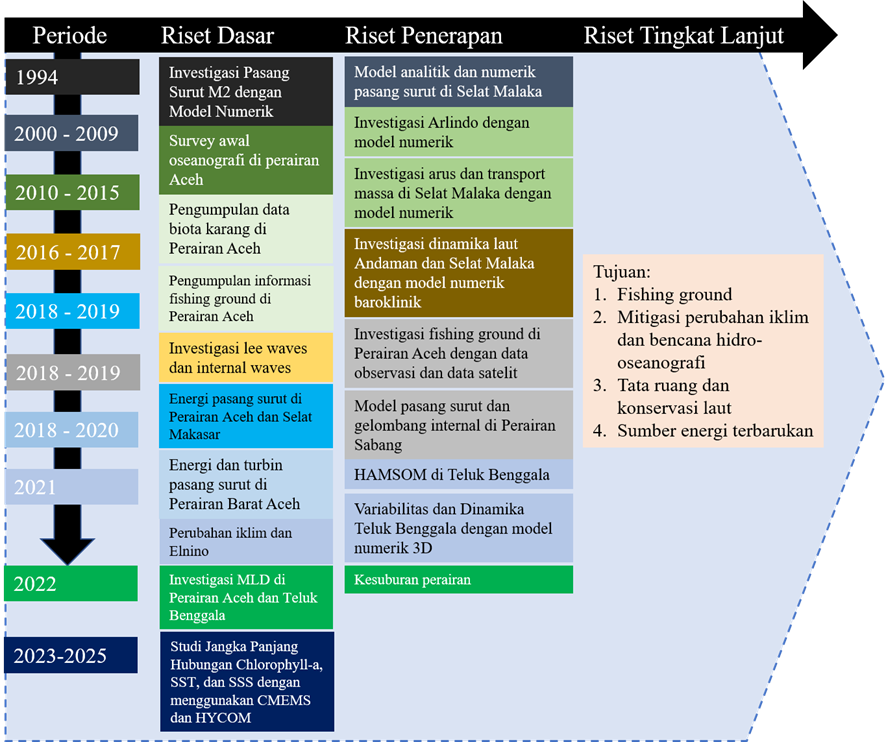
\includegraphics[width=12cm]{contents/Figures/Road_Map}
		\caption{\textit{Road Map} Penelitian}
		\label{fig:RM}
	\end{figure}
	
\end{spacing}